% ====================================================================
%+
% SECTION:
%    MW_Halo.tex
%
% CHAPTER:
%    galaxy.tex
%
% ELEVATOR PITCH:
%
%-
% ====================================================================

\section{Mapping the Milky Way Halo}
%\subsection{Mapping the Milky Way Halo}
\def\secname{MW_Halo}\label{sec:\secname}

\credit{akvivas}, \credit{ctslater}, \credit{dnidever}, \credit{bethwillman}

The study of the halo of the Milky Way is of the highest importance,
not only to understand the formation and early evolution of our own
galaxy, but also to test current models of hierarchical galaxy
formation. LSST will provide an unprecedented combination of area,
depth, wavelength range and long time-baseline for imaging data,
allowing detailed studies of the present-day structure of this old
Galactic component. More detail on each of these tracer populations,
and the general scientific motivations for studies of the Milky Way
halo with LSST, can be found in \citet{2009arXiv0912.0201L}. Here we
focus our attention on halo investigations using three tracer
populations. While we anticipate more cases will be developed and
compared between strategy choices, we have selected populations here
that illustrate many of the most important challenges..
%We focus here on three investigations of the Halo to be
%pursued with LSST data.
We describe the figures of merit (and the
diagnostic metrics on which they depend) that will allow quantitative
assessment of the impact of the choice of observing strategy on the
constraints LSST will afford.
%We expect more projects will join later.  % WIC - not sure what this meant.
We first briefly discuss the use of three main population tracers to
chart the halo population. More detail on each of these tracer
populations, and the general scientific motivations for studies of the
Milky Way halo with LSST, can be found in \citet{2009arXiv0912.0201L}.

{\it 1. RR Lyrae stars} have been known for several decades as
excellent tracers of the halo population. They are not only old stars
($>10$ Gyrs) but they are also excellent standard candles that allow
construction of three-dimensional maps. RR Lyrae stars have been used
to survey Milky Way halo populations extending out to
%The halo of the Milky Way has
%been now surveyed in a very large extension up to
$\sim 60-80$ kpc from the Galactic center \citep[][among
  others]{drake13a,drake13b,zinn14,torrealba15}. Beyond $\sim 80$~kpc,
the halo is mostly uncharted territory.

The RR Lyrae surveys suggest the halo is filled with substructures
(clumps of elevated stellar density) which are usually interpreted as
debris from destroyed satellite galaxies. This substructure overlies a
smooth component in the distribution of RR Lyrae stars, whose number density is well-described by a power law in galactocentric distance,
%which is well described
%with a power-law in the mean number density of RR Lyrae stars as a
%function of galactocentric distance,
steepening at radii $\gtrsim 30$ kpc \citep{zinn14}.  Thus, beyond
$\sim 60$ kpc, few field RR Lyrae stars are expected. However, we
presume that any RR Lyrae star beyond this distance may be part of
either debris material or distant low-luminosity satellite galaxies
% of low luminosity
that have been escaped detection until now \citep{sesar14,baker15}.
LCDM models predict debris as far as $0.5$~Mpc from the galactic
center This is the territory that will be explored by LSST.

{\it 2. Red giant stars} can similarly be used to trace the structure
of the halo up to large distances. They have the advantage of being
bright and are numerous compared to the RR Lyrae stars.

{\it 3. Main sequence stars}, although less luminous than RR Lyraes or
Red Giants, are so much more numerous that statistical studies can be
pursued in a manner not generally possible for those populations.
%Fainter than these two tracers, main
%sequence stars stand up as a tool for studying the Halo. They are the
%most numerous type of stars available and statistical studies are
%possible.
Using the technique of photometric metallicities \citep{ivezic08}, the
Sloan Digital Sky Survey (SDSS) provided unprecedented maps of the
metallicity distribution up to $\sim 10$ kpc from the Galactic center,
unveiling not only the mean metallicity distribution of the halo but
also, sub-structures within the halo. LSST will extend these studies
all the way to the outermost parts of the Galaxy.
%This kind of works will be extended to the outermost parts of the
%Galaxy with LSST data.

% --------------------------------------------------------------------

% \subsection{Target measurements and discoveries}
\subsubsection{Target measurements and discoveries}
\label{sec:\secname:MW_Halo_targets}

Accurate measurement of these three tracer populations implies the following requirements:

%The three projects just described require the discovery and/or measurement of t%he following
%type of objects:

\begin{itemize}

\item[1.] RR Lyrae stars: These are bright horizontal-branch variable
  stars with periods between 0.2 to 1.0 days and large amplitudes,
  particularly in the bluer bandpasses (g amplitudes $0.5 -
  1.5$~mag). \citet{2012AJ....144....9O} made an intensive search for
  RR Lyrae stars in simulated LSST data and reached to the conclusion
  that this type of stars can be recovered to distances $\sim 600$
  kpc. A similar procedure can now be performed using MAF to directly
  compare LSST cadence scenarios to each other.
  %and current cadence scenarios.
  Chapter \ref{chp:variables} discusses the
  discovery metrics for variable stars including RR Lyrae
  stars. However, optimal recovery may involve more complex metrics
  involving the simultaneous use of multi-band time series
  \citep{vanderplas15,vivas16}. Besides recovery of variable stars,
  stars, red-wavelength mean magnitudes $z$~and $y$ are particularly
  valuable since they provide the most accurate distance indicators.
  %valuable measurement to track for studies in the halo is the
  %infrared mean magnitudes z and y
\citep{caceres08}.

\item[2.] Main sequence stars: lacking any distinguishable variability, the
challenge in selecting a large and clean sample of main sequence stars comes
from tremendous number of small and nearly-unresolved galaxies present at
faint magnitudes. Precise star/galaxy separation is thus the limiting factor
on the useful depth of the main sequence sample. In addition to identifying
dwarfs, using dwarfs to map the metallicity distribution of the halo requires
precise $u$-band data, since it exhibits the strongest metallicity dependence of
the LSST filters.

\item[3.] Red Giants: due to their intrinsic luminosity, the Red Giants will sample
a far larger volume than main sequence stars at similar apparent magnitudes. However, they must first be identified and separated from the very numerous main
sequence stars present in the foreground. A gravity-sensitive photometric index can
be used for separating efficiently giants from dwarfs. The $u$-band magnitude is essential for such an index, so
%is
%an essential ingredient in this process, and
the behavior of the $u$-band limiting magnitude must therefore be charted under the various observational strategies under consideration.
% and it is necessary to follow-up
%the behavior of the u limiting magnitude under different observational
%strategies.
\autoref{fig-MW-giants} shows the distance that can be reached
by M-giants of different metallicities assuming limiting magnitude $u = 26.0$.
%-band limiting magnitude of 26.0..

\end{itemize}

\begin{figure}[h]
\begin{center}
  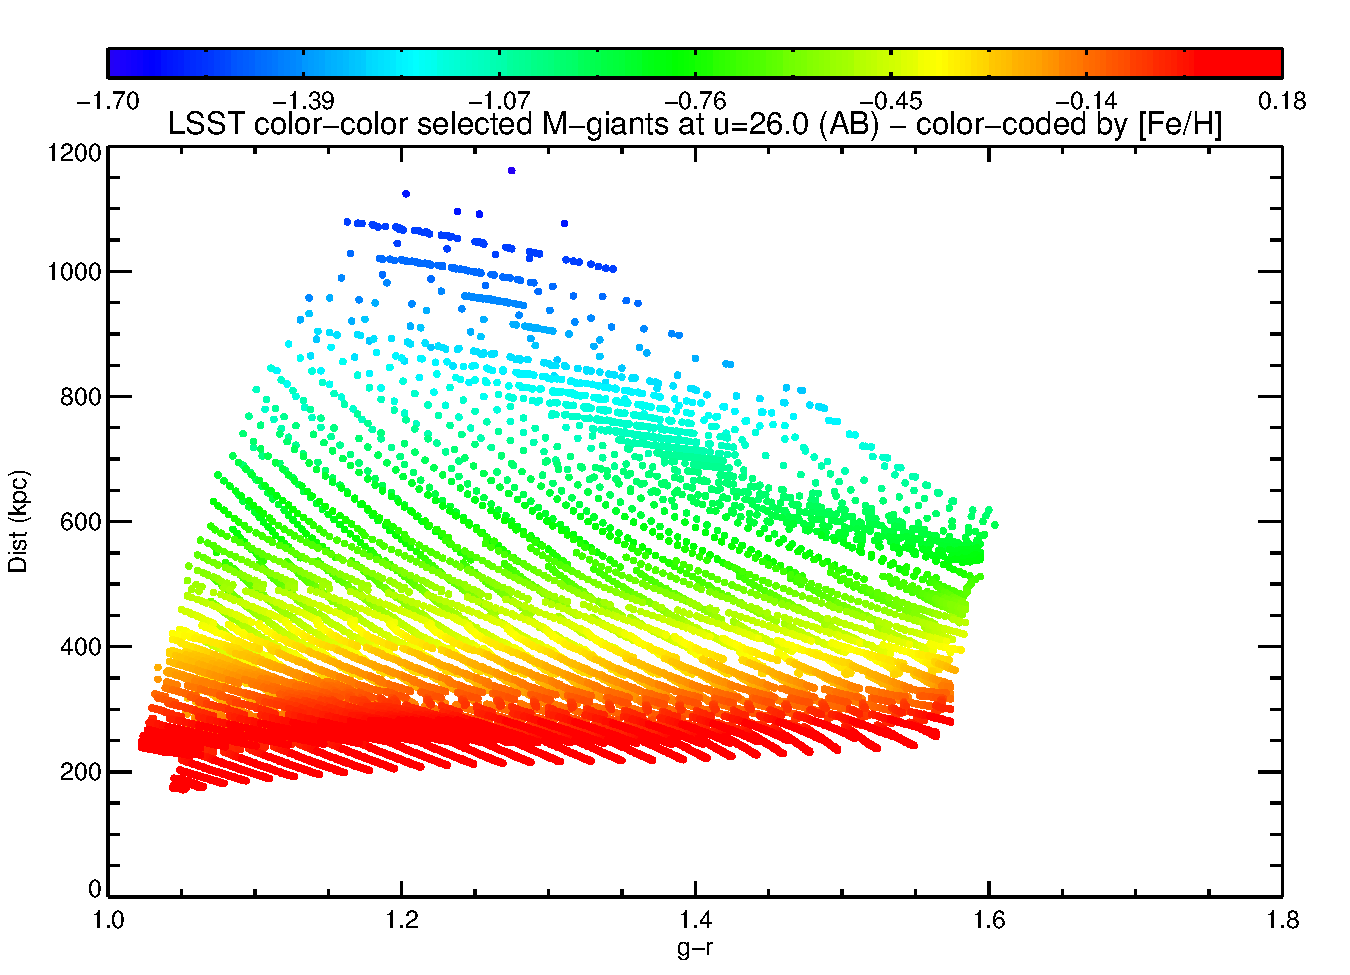
\includegraphics[scale=0.5]{./figs/milkyway/lsst_mgiants_grdist.pdf}
  \caption{Distance to which red giant stars can be identified in the galactic halo assuming a limiting magnitude
  of u=26.0. The color code scales with the metallicity of the stars. More metal-poor stars can be
  detected to farther distances. \label{fig-MW-giants}}
\end{center}
\end{figure}


% --------------------------------------------------------------------

% \subsection{Metrics}
\subsubsection{Metrics}
\label{sec:\secname:MW_Halo_metrics}

\textbf{Star-Galaxy Separation:} For main sequence stars, the useful depth of
the survey will likely not be the photometric detection limit, but will instead
be set by the ability to differentiate stars from unresolved background
galaxies. Towards faint magnitudes the contamination by galaxies worsens
significantly for several reasons: the number of galaxies is rising
substantially, the angular size of galaxies is shrinking, and our ability to
distinguish stars from marginally resolved galaxies diminishes for faint
sources simply due to photon statistics. While the fundamental properties of
the contaminant sources are beyond our control, our ability to reject these
sources depends on survey parameters which do vary with the choice of observing strategy, such as the distribution of seeing across
visits and the depth of these visits.

We are currently in the process of developing a metric that will estimate our
ability to separate stars and galaxies for any observation depth and seeing
conditions. This requires both an understanding of how images of a source are
measured and classified as either a star or galaxy, and how the population of
stars and galaxies vary in number and size (for galaxies) with depth. Our model
uses the distribution of galaxies in size and number, derived from HST COSMOS
observations, along with a fully Bayesian model decision formalism to compute
the expected completeness and contamination in star-galaxy separation.
Computationally, for each position in the survey footprint we interpolate the
results from that work on a grid in seeing, galaxy size, and coadd depth, then
integrate over the distribution of galaxy sizes. This modeling process is
currently being verified against existing surveys, and will be incorporated into
the observing strategy study at a later date.

%This is a diagnostic metric and some of the higher level metrics
%described below will depend on it.
Some of the higher-level figures of merit described below will depend on this star/galaxy separation diagnostic metric.

\textbf{Distance to the farthest RR Lyrae stars:} This metric charts our ability to
recover an RR Lyrae star from LSST data as a function of its distance. An RR Lyrae star may be
considered as recovered if its period and amplitude are within 10\% of the intrinsic values.
The procedure followed by \citet{2012AJ....144....9O} is a good example on how this can be
achieved. They built a large number of synthetic light curves spanning the properties of
known RR Lyrae stars and ``observed'' them with the cadence given by the OpSim runs
available at that time. Anticipated improvements over this previous work include the use
of simultaneous multi-band information to recover periods \citep[e.g.,][]{vanderplas15,vivas16}.

However, a first look into this problem using MAF can be achieved
by simplifying the procedure and only test if a star with period 0.55 days (the mean period for
RR Lyrae stars) can be recovered by metrics already available in MAF.
Then, distance can be calculated using the mean magnitude of the recovered RR Lyrae stars
(in the reddest bands available to LSST) and the interstellar extinction at that point of the sky (maps are available
now in MAF).  This metric should compute the largest distance that can be measured with a 10\% precision
at which certain percentage of RR
Lyrae stars (eg. 80\%) can be recovered by LSST. It is expected that the results
of this metric at low galactic latitudes will be largely dependent on the chosen observational
strategy (through variations in cadence towards the Plane).
%(how sparse will the cadence be  in the galactic plane).

A reasonable Figure of Merit for this sub-project is the volume of the
halo within RR Lyrae stars  can be recovered. Similarly, another Figure
of Merit would be the fraction of the Galactic thick disk's volume that
can be traced by RR Lyrae stars.

\textbf{Distance to the farthest main sequence stars and giant stars:}
Since variability is not the signal property for these tracer
populations, metrics are somewhat simpler than for the RR Lyrae.
%Being non-variable objects,
%the metrics for these objects are somewhat simpler than for the RR Lyrae. and
Here the distance metric requires the determination of the limiting $u$-band
magnitude
%(in u band)
for which galaxy/star separation is reliable to a certain level. In
these cases, distances depend on metallicity. Then, a figure of merit is
the volume of the halo mapped with stars within a specified metallicity
range.


% % --------------------------------------------------------------------
%
% \subsection{OpSim Analysis}
% \label{sec:\secname:MW_Halo_analysis}
%
% \autoref{tab_SummaryMWHalo} summarizes the science Figures of Merit
% for the Milky Way halo science cases for LSST.
% %OpSim analysis for this
% %Section will be summarized in that Table;
% At the present date (April
% 2016) placeholder rows are given for the FoM's. We welcome input from readers.
% %Input from the readers
% %is welcome!
%
% %%% SUMMARY TABLE FOR THIS SUBSECTION
%
% \begin{table}
%   \begin{tabular}{l|p{6cm}|c|c|c|c|p{5cm}}
%     FoM & Brief description & {\rotatebox{90}{\opsimdbref{db:baseCadence} }} & {\rotatebox{90}{\opsimdbref{db:opstwoPS} }} & {\rotatebox{90}{\scriptsize{\tt astro\_lsst\_01\_1004}  }} &  {\rotatebox{90}{future run 2}} & Notes \\
%     \hline
%     1.1. & \footnotesize{Survey volume to RR Lyraes}      & - & - & - & - & \footnotesize{Volume within which the distance to a template RR Lyrae star can be estimated to 10\% uncertainty.} \\
%     1.2. & \footnotesize{Survey volume to Main Sequence tracers} & - & - & - & - & \footnotesize{(Including star-galaxy separation)} \\
%     1.3. & \footnotesize{Survey volume to Red Giants} & - & - & - & - & - \\
% %    2.1. & \footnotesize{Completeness of metallicity sub-structure recovery as a function of distance} & - & - & - & - & \footnotesize{Over all three tracer populations?} \\
% %    3.1. & \footnotesize{Uncertainty and bias in age distribution parameterization of the main Halo population} & - & - & - & - & - \\
% %    3.2. & \footnotesize{Uncertainty and bias in the population fraction identified correctly with each halo component} & - & - & - & - & \footnotesize{Some overlap with Halo astrometry FoM?} \\
% \end{tabular}
% \caption{Summary of figures-of-merit (FoMs) for the Galactic Halo science cases. The best value of each FoM is indicated in bold. Runs \opsimdbref{db:baseCadence} and \opsimdbref{db:opstwoPS} refer to the Baseline and PanSTARRS-like strategies, respectively. Column {\tt astro\_lsst\_01\_1004} refers to a recently-completed OpSim run that includes the Plane in Wide-Fast-Deep observations. See Section \ref{sec:MW_Halo}.}
% \label{tab_SummaryMWHalo}
% \end{table}
%
%
% --------------------------------------------------------------------

%\subsection{Discussion}
%\label{sec:\secname:MW_Halo_discussion}

%Discussion: what risks have been identified? What suggestions could be
%made to improve this science project's figure of merit, and mitigate
%the identified risks?


% ====================================================================

\navigationbar
